\chapter{Simulation von Streubildern}
Es ist sinnvoll, die Evaluierung von Rekonstruktionsansätzen zunächst mit synthetischen Streubilder durchzuführen, da so das ideale Rekonstruktionsergebnis bekannt ist und für einen direkten optischen Vergleich zur Verfügung steht\footnote{\textit{"`To our
	knowledge there is no reliable objective metric for image quality. Ultimately, the quality
	comparison between algorithms is based on what looks good to the user"'}, D. R. Luke in der Vorstellung des \textit{RAAR}-Algorithmus~\cite{luke2004}.}. 
Für das Problem der Berechnung synthetischer Streubilder existieren verschiedene Lösungsansätze: Neben den verbreiteten Methoden \textit{DDA} und \textit{FDTD}, die in allen Raumrichtungen Berechnungspunkte in einem Abstand deutlich geringer als die Wellenlänge benötigen, kann die 3D-Fouriertransformierte, die auch mit weniger Punkten noch valide Ergebnisse liefern kann, genutzt werden~\cite{kunz1993,sander2014,hantke2016}. Diese vernachlässigt jedoch Mehrfachstreuung und Absorption und wird ebenfalls durch den Berechnungsaufwand hinsichtlich der Ausmaße der Objekte, deren Streubilder berechnet werden können, limitiert. Von besonderem Interesse sind deshalb die verschiedene schichtweise arbeitende Ansätze, die im Folgenden vorgestellt und bezüglich ihrer Gültigkeit überprüft werden.

\section{Mie-Streuung}
Die Mie-Theorie bietet eine analytische Lösung der Streuung an einer Kugel in Form einer unendlichen Reihe, basierend auf einer Lösung der Grenzbedingungen für elektromagnetische Wellen~\cite{bohren1983}. Diese unendliche Reihe lässt sich näherungsweise numerisch berechnen (Details siehe \fref{app:mie}). Eine vektorisierte Version dieser Berechnung ist in den auf Mätzler~\cite{maetzler2002} basierenden Matlab Funktionen \texttt{simulation/mie.m} für winkelabhängige Radialprofile sowie \texttt{simulation/mie\_scatter.m} für Streubilder implementiert. Diese für eine homogene Kugel im Vakuum korrekte Lösung dient im Rahmen dieser Arbeit der Verifizierung der Simulationsverfahren.

\section{Projektions-Näherung}
	
Um dreidimensionale Streuobjekte durch zweidimensionale Blenden zu nähern, lässt sich die Projektion ihrer Dichteverteilung auf eine Ebene direkt hinter ihnen betrachten. In Näherung verhält sich eine elektromagnetische Welle nach Durchlaufen eines hinreichend dünnen Objektes gleich wie nach Durchlaufen einer Blende mit dieser durch Projektion gewonnenen Absorption und Refraktion, sodass in Fraunhofer-Fernfeldnäherung das Streubild durch die zweidimensionale Fouriertransformierte der Projektion genähert werden kann.
	
Für eine kreisförmige Blende existiert eine analytische Darstellung der Fouriertransformation in Form der sogenannten Airy-Scheibe. Das Streubild eines Objektes mit kreisförmiger Projektion lässt sich somit mittels der Besselfunktion 1. Ordnung $J_n$ als
\begin{equation}
	I(\theta) \propto \left ( \frac{2 J_1(kr \sin \theta)}{kr \sin \theta} \right )^2 
\end{equation}
nähern~\cite{born1980}. Für nicht kreisförmige Projektionen der Dichte lässt sich die Fouriertransformation diskret numerisch auswerten.

Im Weiteren wird die Projektion der Dichte und anschließende diskrete Fouriertransformation dieser als \textit{Projektions-Näherung} bezeichnet. Diese Näherung wird bei dem Vergleich der Simulationsansätze mit betrachtet aufgrund des geringen Rechenaufwandes und der Möglichkeit, auch nicht-kugelförmige Objekte zu behandeln (im Gegensatz zur Rayleigh-Gans-Näherung).


\section{Multislice Fouriertransformation}
Das Grundprinzip der in mehreren Schichten arbeitenden \textit{Multislice} Algorithmen ist in \fref{fig:multislice_prinzip} dargestellt: Die Streuobjekte (in diesem Beispiel eine Kugel) werden zunächst in eine quaderförmige \textit{Szene} eingebettet und diskretisiert. Hierbei können unterschiedliche Auflösungen in x,y und z-Richtung gewählt werden. Bei der Simulation werden nun einzelne Schichten gleichen z-Wertes betrachtet.
\begin{figure}
	\centering
	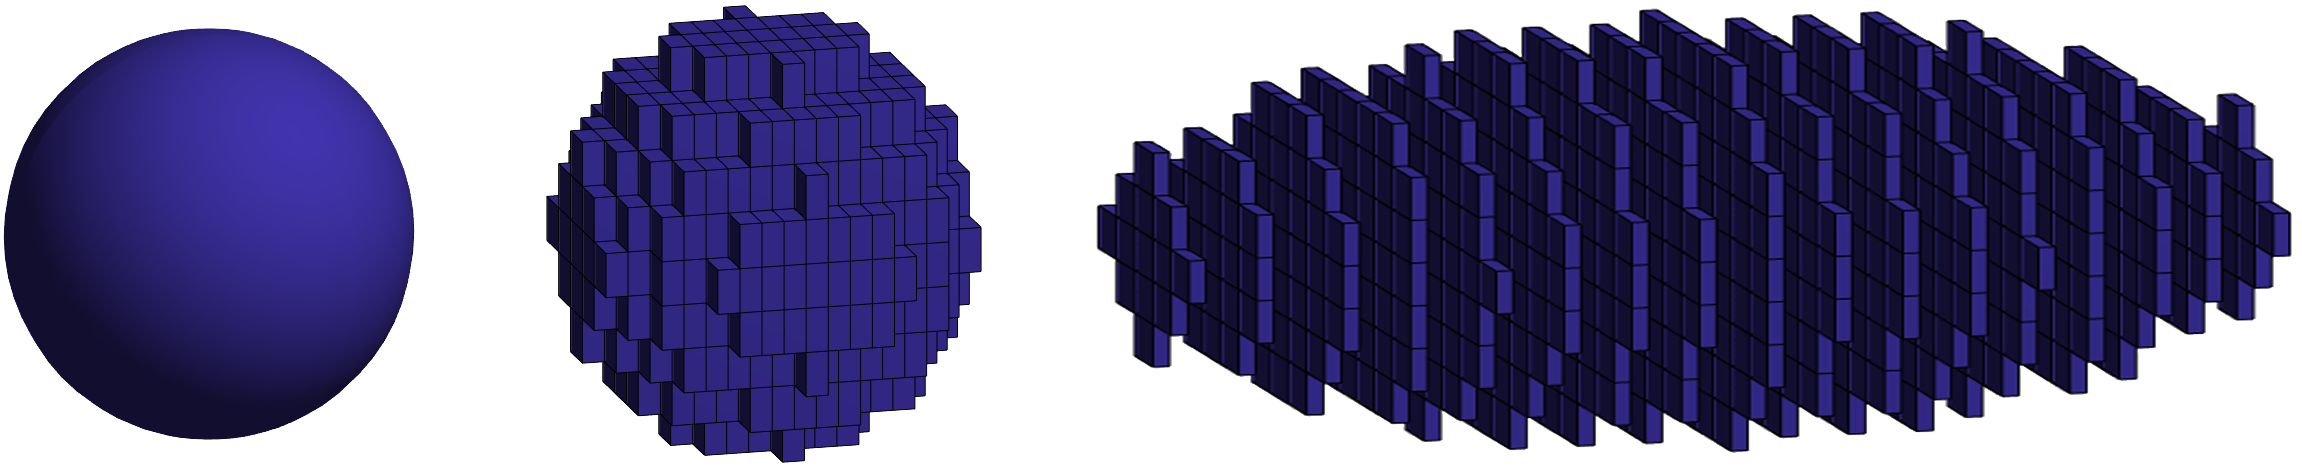
\includegraphics[width=1\textwidth]{images/multislice_sphere.png}
	\caption[Prinzip Multislice]{Prinzip der Multislice-Simulation: Das zu simulierende Streuobjekt (in diesem Fall eine einfache Kugel) wird in eine quaderförmige Szene eingebettet (wobei für die Berechnung eine größere x,y-Ausdehnung als z-Ausdehnung gewählt wird) und diskretisiert. Üblicherweise wird hierbei eine feinere Auflösung $\Delta z$ in Strahlrichtung gewählt. Bei der Simulation werden nun einzelne Schichten betrachtet.}
	\label{fig:multislice_prinzip}
\end{figure} 

Einer dieser Algorithmen ist die \textit{Multislice Fouriertransformation (MSFT)}. Nach \fref{eq:born} gilt in der ersten Bornschen Näherung für die Amplitude der gestreuten Welle
\begin{equation}
	\phi\propto\int \delta\eta(\vec{r}) e^{-i\vec{q}\cdot \vec{r}} \dif \vec{r} \, .
\end{equation}
Um die Komplexität zu reduzieren, wird nun versucht auf eine schichtweise Berechnung überzugehen: Wird das Skalarprodukt $\vec{q}\cdot \vec{r}=xq_x+yq_y+zq_z$ ausgeschrieben und die Integration über $x$ und $y$ als zweidimensionale Fouriertransformation interpretiert,
\begin{equation}
	\phi\propto\int \mathscr{F}\left[\delta\eta\right](q_x,q_y,z) e^{-izq_z} \dif z \, ,
\end{equation}

so lässt sich das Integral in z-Richtung als Summe interpretieren:
Aufgrund der Impulserhaltung muss für die Wellenvektoren $\vec{k_0}^2=\vec{k}^2=k^2$ gelten. Nach  \fref{fig:vec_msft} lässt sich der Streuvektor $q$ in einen zum einfallenden Wellenvektor parallelen Anteil $q_\parallel$ sowie einen senkrechten Anteil $q_\perp$ zerlegen,
\begin{align}
	k^2=(k-q_\parallel)^2+q_{\perp}^2                  
	\Leftrightarrow q_\parallel=k-\sqrt{k^2-q_\perp^2} \,.
\end{align}
\begin{figure}
	\centering
	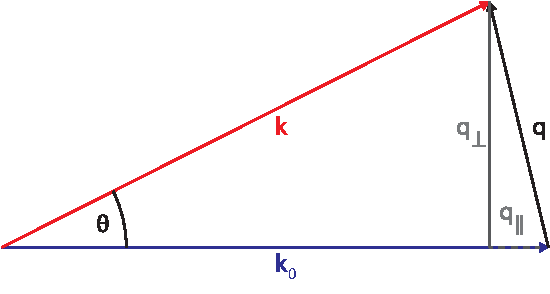
\includegraphics[width=0.5\textwidth]{images/vec_msft.pdf}
	\caption[Vektoren bei MSFT]{Skizze zur Bezeichnung der Vektoren. $\vec{k_{0}}$ und $\vec{k}$ bezeichnen den Wellenvektor der einfallenden bzw. ausfallenden Welle mit dem dazwischenliegenden Winkel $\theta$. $\vec{q}$ bezeichnet den Streuvektor mit einer zu $\vec{k_{0}}$ parallelen ($q_{||}$) und einer senkrechten ($q_\perp$) Komponente.}
	\label{fig:vec_msft}
\end{figure} 

Somit kann $q_z=q_\parallel$ eingesetzt werden und es gilt für die Welle im Fernfeld wie in \fref{fig:slice_msft} illustriert
\begin{equation}
	\label{eq:msft}
	\phi\approx\sum_n{\mathscr{F}\left[\delta\eta\right] e^{-in\delta_z\left(k-\sqrt{k^2-q_\perp^2}\right) }} \, .
\end{equation}

\fref{eq:msft} beschreibt einen Algorithmus um das Streubild eines dreidimensionalen Objektes im Fernfeld schichtweise in der ersten Bornschen Näherung zu berechnen~\cite{barke2015}. 

\begin{figure}
	\centering
	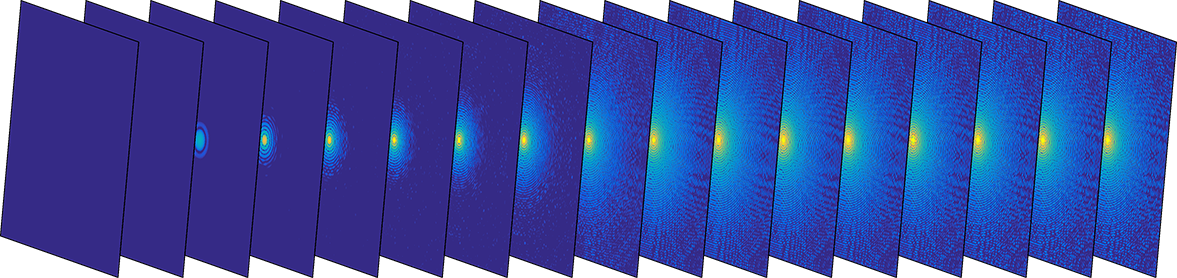
\includegraphics[width=1\textwidth]{images/slice_msft.png}
	\caption[Illustration MSFT]{Illustration zur MSFT: Das Streubild wird berechnet indem schichtweise der jeweilige Beitrag der Bornschen Näherung phasenkorrekt aufaddiert wird (dargestellt von links nach rechts). Das Bild rechts außen ist somit das Streubild des Objektes und das Ergebnis des Algorithmus.}
	\label{fig:slice_msft}
\end{figure} 

Bei dieser Methode wird Mehrfachstreuung vollständig ignoriert. Durch nachträgliches Einführen eines zusätzlichen Faktors, der die Absorption und Phasenänderung der Welle beim Durchlaufen des Objektes beschreibt, ließe sich nachträglich eine grobe Näherung für Absorptionseffekte einführen, die in einigen Fällen die subjektive Qualität der Simulation zu verbessern scheint~\cite{barke2015}. Da zum Einen die Gültigkeit dieser Absorptionsnäherung nicht direkt abgeschätzt werden kann und sie zum Anderen nicht in allen Fällen die Güte der Simulation verbessert, ist im Weiteren mit \textit{MSFT} die Methode ohne diese Korrektur bezeichnet~\cite{fennel}.
Eine Implementierung des MSFT-Algorithmus mit optionaler Absorptionskorrektur liegt in \texttt{simulation/msft.m} vor. 

\section{Multislice Propagation}
Ein alternatives Verfahren zur Simulation von Streubildern ist in der Literatur als \textit{Multislice Propagation} oder \textit{Beam Propagation} bekannt~\cite{hare1994,cowley1957}. Bei diesem in \fref{fig:multislice} skizzierten Verfahren wird zunächst die Szene in einzelne Schichten mit dem Abstand $\Delta z$ zerlegt. Die Ausbreitung der in die Szene einfallenden ebenen Welle wird nun genähert durch eine Vakuumpropagation von Schicht zu Schicht nach \textit{Angular Spectrum Propagation} im Hybridraum\footnote{Die Näherung der Vakuumausbreitung durch einen Fresnel-Propagator bringt gegenüber der korrekten Berechnung über die Angular Spectrum Propagation keine numerischen Vorteile. Aus diesem Grund wird im Gegensatz zu~\cite{hare1994} auf diese Näherung verzichtet.},
\begin{equation}
	\bar{\phi}\left(q_x,q_y,z+\Delta z\right)=\bar{\phi}(z)e^{i\Delta z\sqrt{k^2-(q_x+q_y)^2}} \, ,
\end{equation}
sowie durch eine Wechselwirkung mit der Materie der Schicht in einer einzelnen Ebene im Realraum
\begin{equation}
	\phi(x,y,z+\Delta z)=\phi e^{i\delta n\left(z\right) \Delta z} \, .
\end{equation}
\begin{figure}
	\centering
	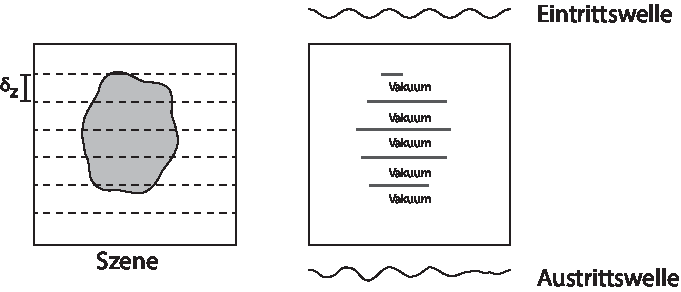
\includegraphics[width=0.9\textwidth]{images/multislice.pdf}
	\caption[Prinzip Multislice Propagation]{Prinzip der Multislice Propagation: Die Szene wird in einzelne Schichten zerlegt und die Wechselwirkung mit der Materie jeder einzelnen Schicht in auf eine in dieser Schicht liegenden Ebene reduziert. Zwischen diesen Ebenen wird eine Vakuumpropagation angewendet.}
	\label{fig:multislice}
\end{figure} 	

Bei diesem Verfahren wird die Annahme getroffen, dass  innerhalb einer Schicht die örtliche Verteilung der Materie konstant ist, sowie die durch die Propagation bedingte Veränderung innerhalb von $\Delta z$ ausreichend klein ist, sodass keine Anteile der Wellenfront innerhalb einer Schicht unterschiedliche Brechzahlen durchlaufen~\cite{hare1994}. Dies kann durch ein hinreichend kleines $\Delta z$ gewährleistet werden. 
Des Weiteren wird bei der Wechselwirkung mit der Materie der Winkel mit dem ein Anteil der Wellenfront durch die Materie läuft vernachlässigt: Bei Anteilen der Welle, die durch vorangegangene Streueffekte bereits in einem deutlichen Winkel die Szene durchlaufen, wird genähert, dass ihr Weg durch die Materie gleich lang wie der Weg von nicht gestreuten Anteilen ist. Somit wird Mehrfachstreuung zwar mitberücksichtigt, jedoch nur näherungsweise.
	
Der Algorithmus zur Berechnung der Austrittswelle, d.h. der Welle hinter der Szene bzw. dem Streuobjekt, ist somit die iterative Anwendung von
\begin{equation}
	\label{eq:multislice}
	\Phi(z+\Delta z)= e^{i\delta n\left(z\right) \Delta z}\mathscr{F}^{-1}\left[e^{i\Delta z\sqrt{k^2-(q_x+q_y)^2}}\mathscr{F}\left[\Phi(z)\right]\right] \,.
\end{equation}
Dies ist in \fref{fig:slice_multislice} am Beispiel der Austrittswelle hinter einer Kugel illustriert.

Ist die Austrittswelle bekannt, so ist die weitere Ausbreitung zum Detektor eine Vakuumpropagation, die sich entweder mittels \textit{Angular Spectrum Propagation} berechnen, oder durch eine einfache Fouriertransformation in Fraunhofer-Näherung bestimmen lässt. Ersteres Verfahren hat den Nachteil, das es bei einer numerischen Implementierung im Bereich der Szene die gleiche räumliche Rastergröße wie im Bereich des Detektors erfordert. Bei Anwendung der Fernfeldnäherung ist zwar der maximale Winkel, in dem das Streubild berechnet werden kann, von der räumlichen Auflösung der Austrittswelle sowie die Winkelauflösung von der Szenenausdehnung abhängig, dies ist jedoch deutlich praktikabler.
Diese Methode wird im Weiteren als \textit{Multislice Propagation} bezeichnet und ist in \texttt{simulation/multislice.m} implementiert.

\begin{figure}
	\centering
	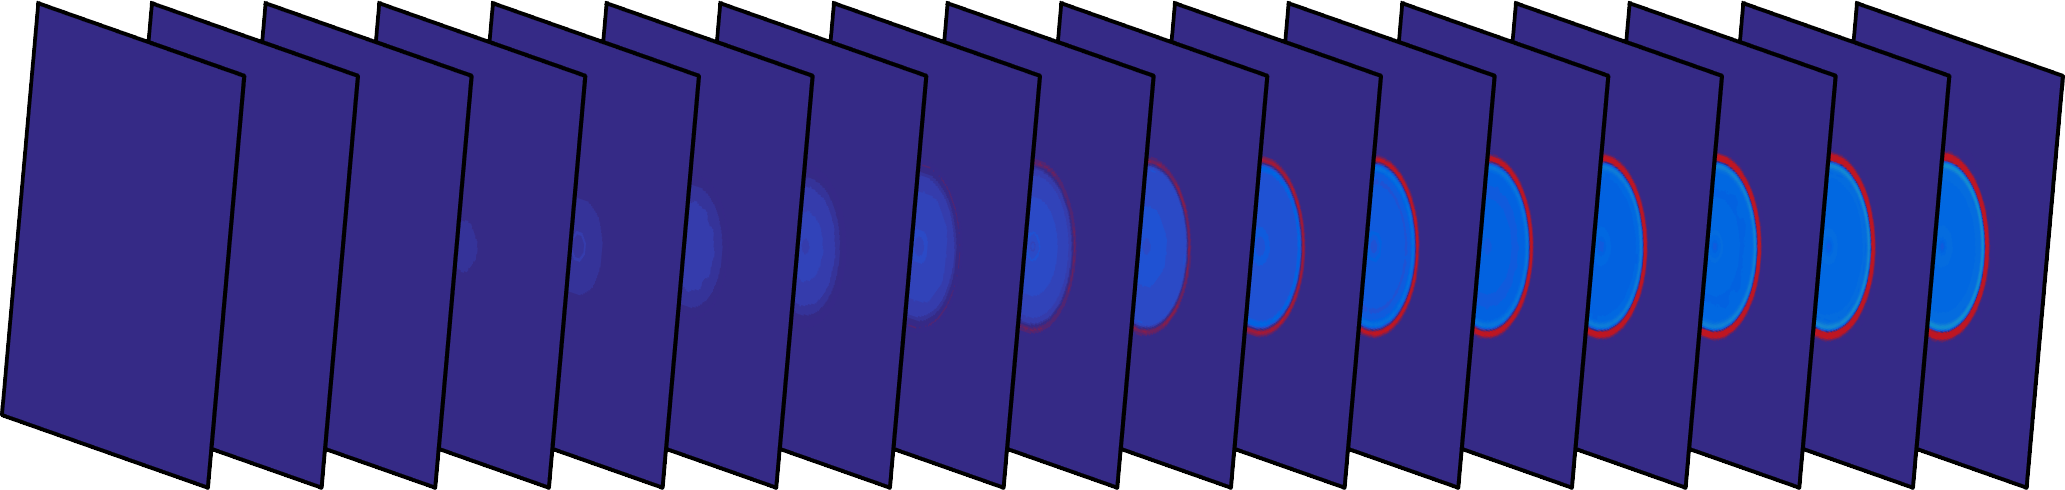
\includegraphics[width=1\textwidth]{images/slice_multislice.png}
	\caption[Illustration Multislice Propagation]{Illustration zur Multislice Propagation: Dargestellt ist der Betrag der komplexen Wellenfront, die Strahlrichtung ist von links nach rechts. Das Bild rechts außen ist die Austrittswelle hinter der Szene und das Ergebnis des Algorithmus.}
	\label{fig:slice_multislice}
\end{figure} 
	
\section{Thibaults Multislice}
Thibault stellt in~\cite{thibault2007} einen eigene Formulierung der Multislice-Simulation auf. Ausgehend von der Wellengleichung (\fref{eq:wellengleichung_green})
lässt sich für die Welle im Hybridraum 
\begin{equation}
	\bar{\Phi}(z)=\bar{G}\ast_z\left[\bar{\delta\eta}\ast_{q_\perp} \bar{\Phi}\right]
\end{equation}
mit
\begin{equation}
	\bar{G}=\frac{1}{2\pi}\frac{ik^2}{\sqrt{k^2-q_\perp^2}}e^{iz(q_\parallel-k)}
\end{equation}
aufstellen. Hierbei sind die Faltungsoperatoren mit den Variablen, über die die Faltung durchzuführen ist, indiziert.
Wird nun die Welle bei $\Delta z$ betrachtet, so lässt sich unter Vernachlässigung von Rückstreuung  das Faltungsintegral über $z$ in zwei Integrationsbereiche aufspalten (vom Ursprung bis $\Delta z$ sowie von dort bis ins Unendliche):
\begin{equation}
	\bar{\Phi}(z+\Delta z)=
	\int_{\Delta z}^{\infty} \bar{G}(z')\left[\bar{\delta\eta}\ast_{q_\perp} \bar{\Phi}\right](z+\Delta z-z')\dif z'
	+
	\int_{0}^{\Delta z} \bar{G}(z')\left[\bar{\delta\eta}\ast_{q_\perp} \bar{\Phi}\right](z+\Delta z-z')\dif z' \,.
\end{equation}
Für den ersten Summanden gilt mit einer Substitution ($z'\rightarrow z''+\Delta z$)
\begin{align*}
	  & \stackrel{\hphantom{z'\rightarrow z''+\Delta z}}{\hphantom{=}} 
	\int_{\Delta z}^{\infty} \bar{G}(z')\left[\bar{\delta\eta}\ast_{q_\perp} \bar{\Phi}\right](z+\Delta z-z')\dif z'\\
	  & \stackrel{z'\rightarrow z''+\Delta z}{=}                       
	\int_{0}^{\infty} \bar{G}(z''+\Delta z)\left[\bar{\delta\eta}\ast_{q_\perp} \bar{\Phi}\right](z-z'')\dif z''\\
	  & \stackrel{\hphantom{z'\rightarrow z''+\Delta z}}{=}            
	e^{i\Delta z(q_\parallel-k)}\int_{0}^{\infty} \frac{1}{2\pi}\frac{ik^2}{\sqrt{k^2-q^2_\perp}}e^{iz''(q_\parallel-k)}\left[\bar{\delta\eta}\ast_{q_\perp} \bar{\Phi}\right](z-z'')\dif z''\\
	  & \stackrel{\hphantom{z'\rightarrow z''+\Delta z}}{=}            
	e^{i\Delta z(q_\parallel-k)}\bar{\Phi}(z) \numberthis \,,
\end{align*}
im zweiten Summanden kann für hinreichend kleine $\Delta z$ das Integral gut durch eine Rieman-Obersumme mit einem einzigen Stützpunkt bei $\Delta z$ approximiert werden (der Fehler ist hierbei von der Ordnung $\Delta z$):
\begin{equation}
	\int_{0}^{\Delta z} \bar{G}(z')\left[\bar{\delta\eta}\ast_{q_\perp} \bar{\Phi}\right](z+\Delta z-z')\dif z'
	\approx
	\Delta z \bar{G}(\Delta z)\left[\bar{\delta\eta}\ast_{q_\perp} \bar{\Phi}\right](z) \,.
\end{equation}
Somit lässt sich in Näherung für die Welle bei $z+\Delta z$
\begin{equation}
	\label{eq:thibault}
	\bar{\Phi}(z+\Delta z)
	\approx
	e^{i\Delta z(q_\parallel-k)}
	\left(
	\bar{\Phi}(z)+\frac{\Delta z}{2\pi}\frac{ik^2}{\sqrt{k^2-q^2_\perp}}  \left[\bar{\delta\eta}\ast_{q_\perp} \bar{\Phi}\right](z)
	\right)
\end{equation}
aufstellen. Dies stellt eine iterative Beschreibung der Streuung dar -- ausgehend von $z=0$ kann schrittweise in Einfallsrichtung die Wellengleichung in einer Szene gelöst werden. Somit handelt es sich um einen Algorithmus, der ebenfalls der Kategorie "`Multislice"' zuzuordnen ist. Im Gegensatz zur \textit{Multislice Propagation} findet hier die Wechselwirkung mit der Materie jedoch nicht in Form eines Exponentialfaktor statt, in Kleinwinkelnäherung entspricht \fref{eq:thibault} einer Taylornäherung erster Ordnung in der Exponentialfunktion von \fref{eq:multislice}. Unabhängig von der Gültigkeit der verwendeten Näherungen besitzt \fref{eq:thibault} bei $k^2=q_\perp$ eine Singularität. Aus diesem Grund muss entweder das Raster, in dem die Simulation durchgeführt wird, hinsichtlich der Auflösung in x,y-Richtung so gewählt werden, dass diese Singularität nicht zum Tragen kommt oder nach jedem Simulationsschritt im Fourierraum $\bar{\Phi}(q_x,q_y)$ für $q_x+q_y>k$ auf Null gesetzt werden.
Die numerische Simulation dieser Methode ist in \texttt{simulation/thibault.m} implementiert.


\section{Verifizierung}
Zur Verifizierung der vorgestellten Simulationsalgorithmen und deren numerische Implementierungen eignet sich der Vergleich der berechneten Streubilder hinter Kugeln mit den Ergebnissen aus der Berechnung mittels Mie-Streuung. Der Vergleich wird für verschiedene Brechzahlen und Kugelradien bei einer Wellenlänge von \SI{1}{nm} durchgeführt.

Da ein realer Detektor nicht die Intensitäten bei präzise definierten Winkelpunkten misst, sondern innerhalb eines Areals, ist es zweckmäßig, die simulierte Detektorfläche in quadratische Areale (\textit{Pixel}) zu unterteilen und die Intensität in jedem dieser Areale als gewichtetes Mittel zwischen in dem Areal liegenden Punkten zu betrachten.
Hierbei werden (wie in \fref{fig:average} dargestellt) an den Rändern zwischen zwei Arealen liegende Berechnungspunkte je zur Hälfte in beiden Arealen, in der Ecke zwischen vier Arealen liegende Berechnungspunkte je zu einem Viertel in den vier Arealen berücksichtigt.
Besonders bemerkbar ist dieser Bearbeitungsschritt bei Pixeln die genau in den Intensitätsminima liegen: Ohne die gewichtete Mittlung würde der gesamten Fläche zwischen den Pixeln die Intensität des Minimums zugewiesen werden, auch wenn dessen Breite extrem schmal ist, werden zusätzliche Pixel berechnet und anschließend gewichtet gemittelt, ergibt sich eine korrektere Wiedergabe des tatsächlichen Intensitätsverlaufs. Dies wird sowohl für die mit den verschiedenen Algorithmen simulierten Streubildern als auch für die Mie-Streubilder durchgeführt und einspricht einer einfachen Form des \textit{Antialiasings}, das den Einfluss der diskreten Berechnung verringert.
\begin{figure} %mittelwert
	\centering
	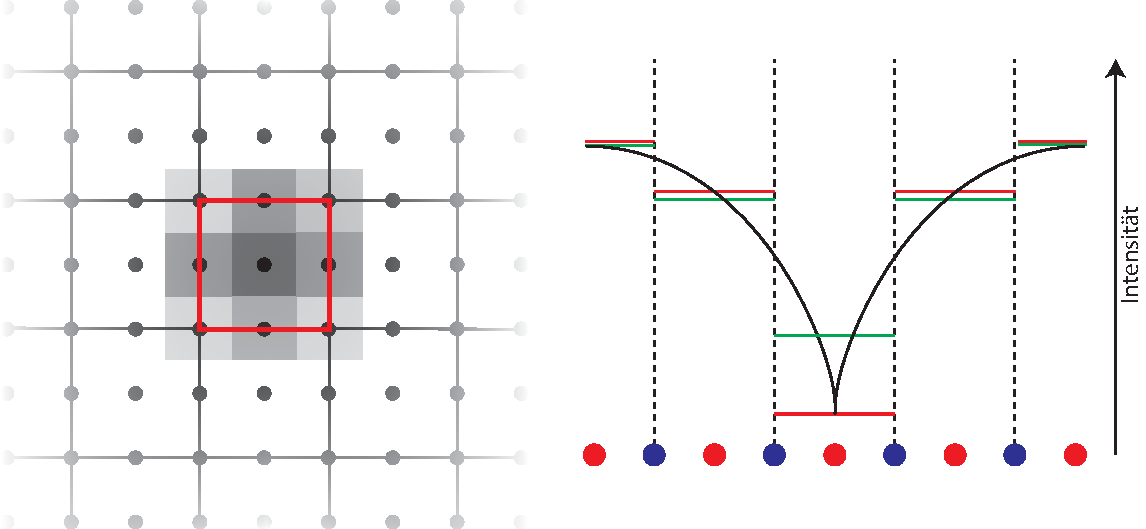
\includegraphics[width=0.9\textwidth]{images/average.pdf}
	\caption[Gewichteter Mittelwert]{Die Verwendung von Überabtastung und gewichteten Mittelwertes bei den Streubildern: Um die Intensität im links rot umrandeten Bereich zu bestimmen, wird die Intensität an den schwarzen Punkten berechnet und ein gewichteter Mittelwert gebildet. Dazu wird die Intensität der vier Randwerte zur Hälfte, die der vier Eckpixel zu einem Viertel in dem umrandeten Bereich mitberücksichtigt. Der Effekt gegenüber einer simplen Berechnung des zentralen Pixels zeigt sich rechts: Wird die Intensität bei einem schwarz dargestellten wahren Intensitätsverlauf nur an den roten Punkten bestimmt, dominiert das Minimum den Intensitätsverlauf. Eine geringere Abweichung ergibt sich bei Berechnung auch an den blauen Punkten und anschließender Bildung des gewichteten Mittelwerts (grün).}
	\label{fig:average}
\end{figure}% 

Anschließend werden die simulierten Streubilder bezüglich ihrer Skalierung auf die Mie-Streubilder normiert. Hierzu wird ein Skalierungsfaktor gesucht, der die mittlere Abweichung der simulierten Streubilder vom jeweiligen Mie-Streubild innerhalb der ersten 10° minimiert. Zur Quantifizierung des Fehlers der simulierten Streubilder wird die relative Abweichung von den Mie-Streubildern betrachtet. Für die \textit{Multislice Propagation} ist in \fref{fig:exitscatter} für einen konkreten Parametersatz exemplarisch Austrittswelle und Streubild dargestellt, die relative Abweichung von Mie ist für diesen Parametersatz in \fref{fig:relerror} für alle Simulationsansätze dargestellt. Aus den rotationssymmetrischen Streubildern können nun Radialprofile der Intensität sowie des relativen Fehlers bestimmt werden um einen besseren Überblick zu erhalten (\fref{fig:profil}). Es ist zu erkennen, dass der relative Fehler in den Datenpunkten, in denen das Mie-Profil ein Minimum hat, aufgrund dessen steilen Verlaufs scharfe, nur 1-2 Datenpunkte umfassende, Maxima annimmt. Um die Güte einer Simulation bei einem bestimmten Radius und Stoffeigenschaften zu quantifizieren, wird deshalb der Median des relativen Fehlers bis 20° Streuwinkel genutzt. So ist es möglich, für die unterschiedlichen Simulationsalgorithmen Bereiche zu bestimmen, in denen sie ausreichend mit der Mie-Theorie übereinstimmen, um sie dort als valide anzusehen. In \fref{fig:variation} wird deutlich, dass bei Werten von $\delta$ bzw. $\beta$ in der Größenordnung bis $10^{-4}$ (die viele Materialien bei \SI{1}{nm} Wellenlänge aufweisen~\cite{henke}) sowohl \textit{Multislice Propagation} und \textit{Thibaults Multislice} als auch \textit{MSFT} valide Ergebnisse liefern -- der mediane Fehler überschreitet 5~\% nicht. Bei größeren Abweichungen der Brechzahl von der Vakuumbrechzahl steigt der mediane Fehler des mittels \textit{MSFT} berechneten Streubildes deutlich an, insbesondere bei großen Radien. Bei diesen kommt es zu deutlich mehr Absorption und Mehrfachstreuung in Vorwärtsrichtung, die bei \textit{MSFT} im Gegensatz zu den beiden anderen Multislice Varianten vollständig ignoriert wird. Der Unterschied zwischen Thibaults Formulierung und der \textit{Multislice Propagation} kann zu einem gewissen Anteil durch die hier verwendete numerische Implementierung von Thibaults Algorithmus begründet sein. Hier besteht weiteres Optimierungspotential bezüglich der Genauigkeit und dem Einfluss von Rundungsfehlern.

\begin{figure} %exitwave und scatter
	\centering
	\begin{subfigure}[b]{0.4\textwidth}
		\setbox1=\hbox{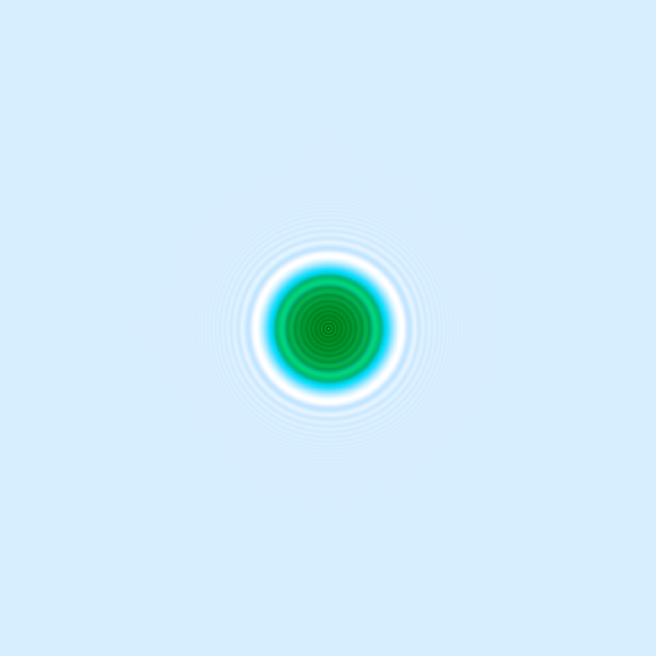
\includegraphics[width=\textwidth]{images/fig_sim_exitwave_multislice-r100-bd1e-3.png}}
		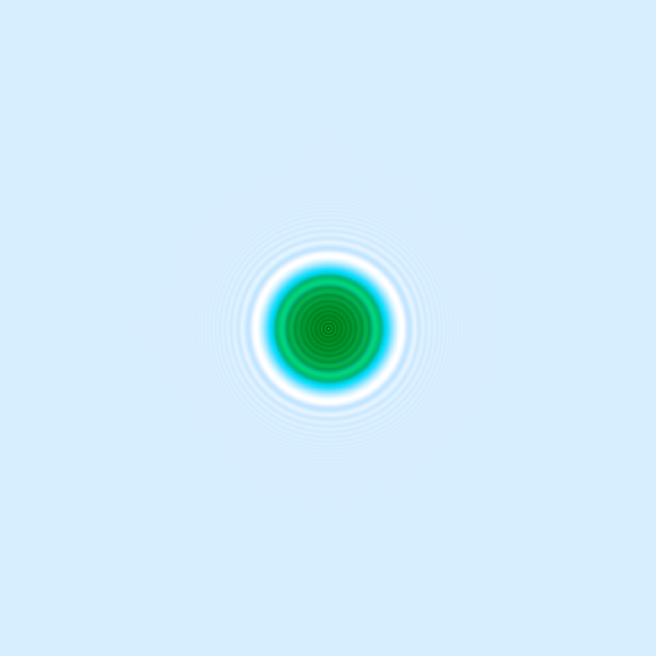
\includegraphics[width=\textwidth]{images/fig_sim_exitwave_multislice-r100-bd1e-3.png}\llap{\makebox[\wd1][l]{\includegraphics[width=0.5\textwidth]{images/fig_sim_exitwave_multislice_cw-r100-bd1e-3.pdf}}}
		\caption{Austrittswelle}
		\label{fig:exitwave}
	\end{subfigure}
	\hspace{1.5cm}
	\begin{subfigure}[b]{0.4\textwidth}
		\setbox1=\hbox{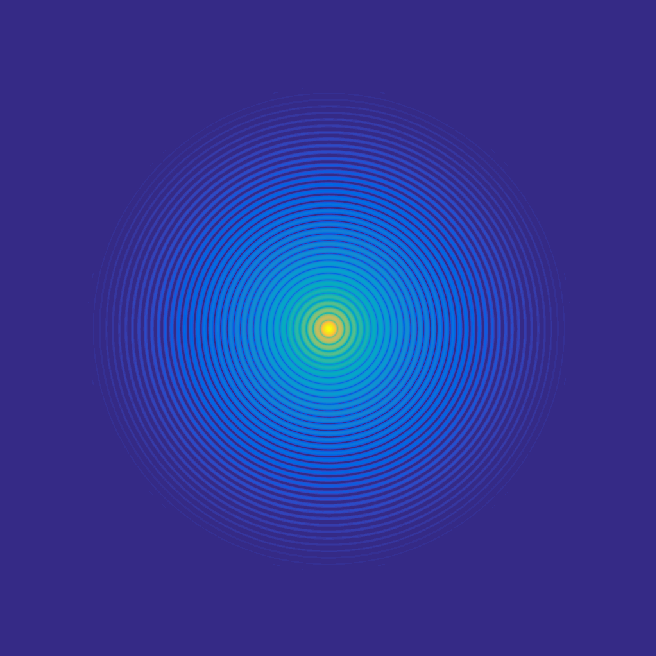
\includegraphics[width=\textwidth]{images/fig_sim_scatter_multislice-r100-bd1e-3.png}}
		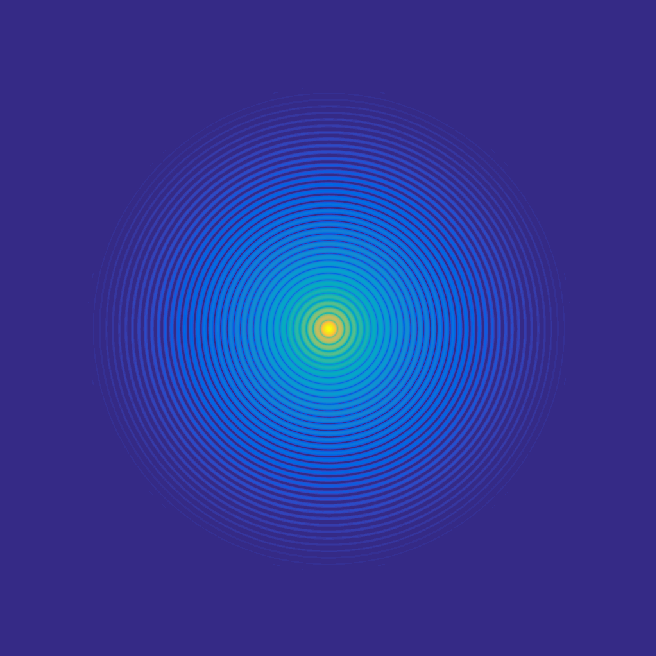
\includegraphics[width=\textwidth]{images/fig_sim_scatter_multislice-r100-bd1e-3.png}\llap{\makebox[\wd1][l]{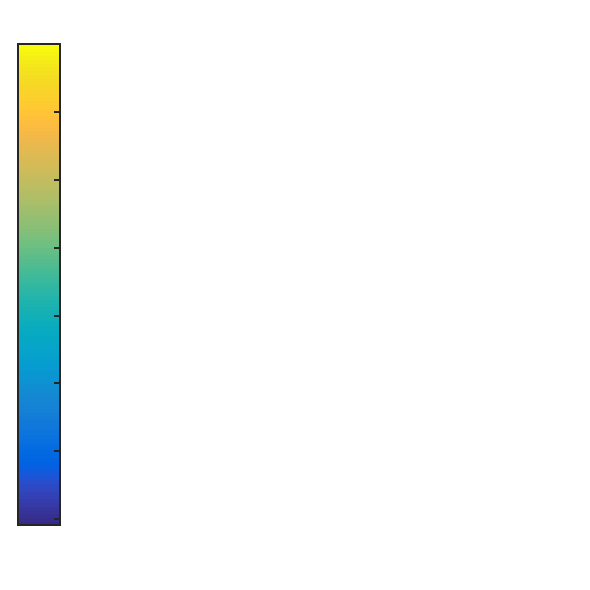
\includegraphics[width=0.5\textwidth]{images/fig_sim_scatter_multislice_cb-r100-bd1e-3.pdf}}}
		\caption{Streubild}
		\label{fig:scatter}
	\end{subfigure}
	\caption[Austrittswelle und Streubild einer Kugel]{Exemplarische Multislice-Propagations Austrittwelle (a) und logarithmiertes Streubild (b) einer Kugel mit Radius \SI{100}{nm} bei $\beta,\delta$=$10^{-3}$. Die relative Intensität der Austrittswelle bezüglich der Eintrittswelle ist über die Helligkeit dargestellt, die Phase über den Farbton. Das Streubild zeigt einen Bereich bis 15°.}
	\label{fig:exitscatter}
\end{figure}%


\begin{figure} %rel error
	\centering
	\begin{subfigure}[b]{0.48\textwidth}
		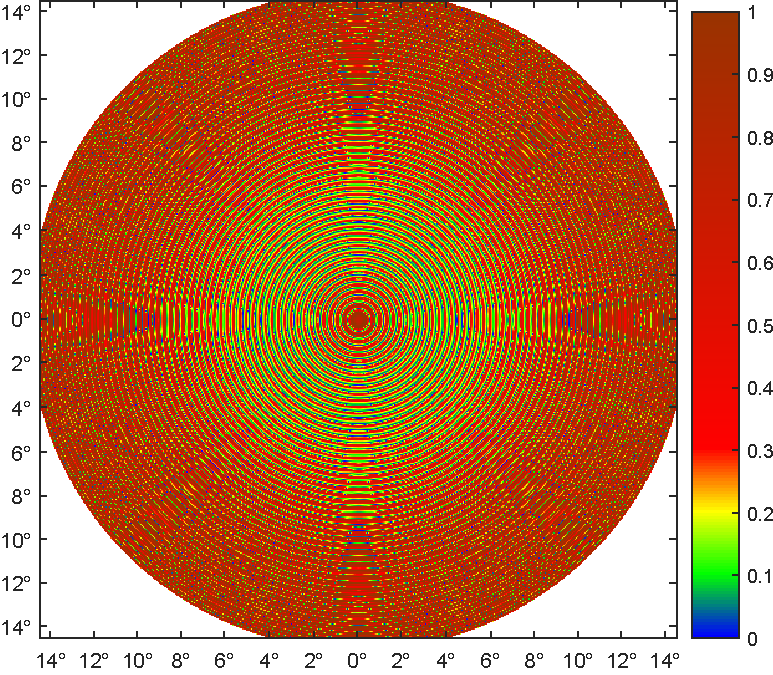
\includegraphics[width=\textwidth]{images/fig_sim_relerror_FTproj-r100-bd1e-3.pdf}
		\subcaption{Projektion}
	\end{subfigure}\hfill
	\begin{subfigure}[b]{0.48\textwidth}
		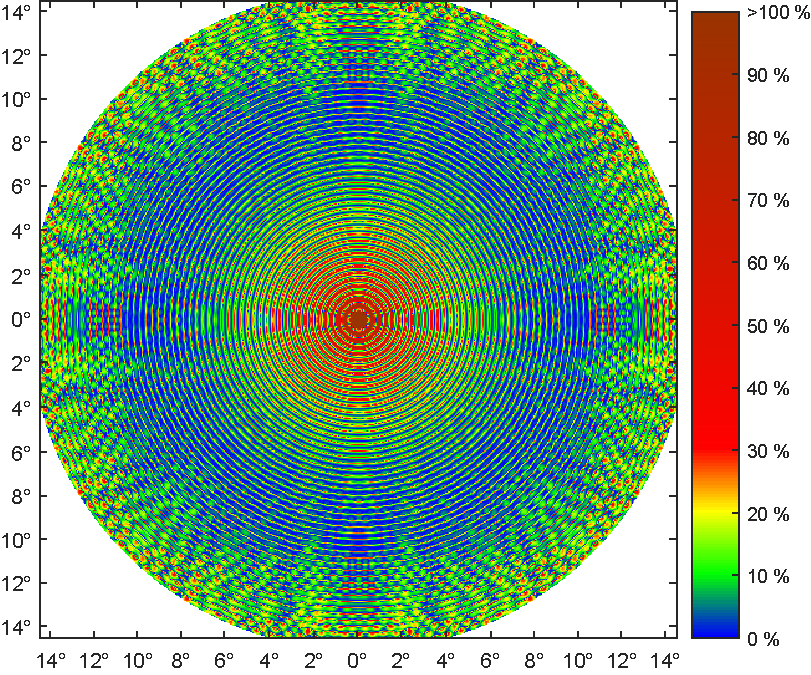
\includegraphics[width=\textwidth]{images/fig_sim_relerror_msft-r100-bd1e-3.pdf}
		\subcaption{MSFT}
	\end{subfigure}
	\par \vspace{1.5\bigskipamount}
	\begin{subfigure}[b]{0.48\textwidth}
		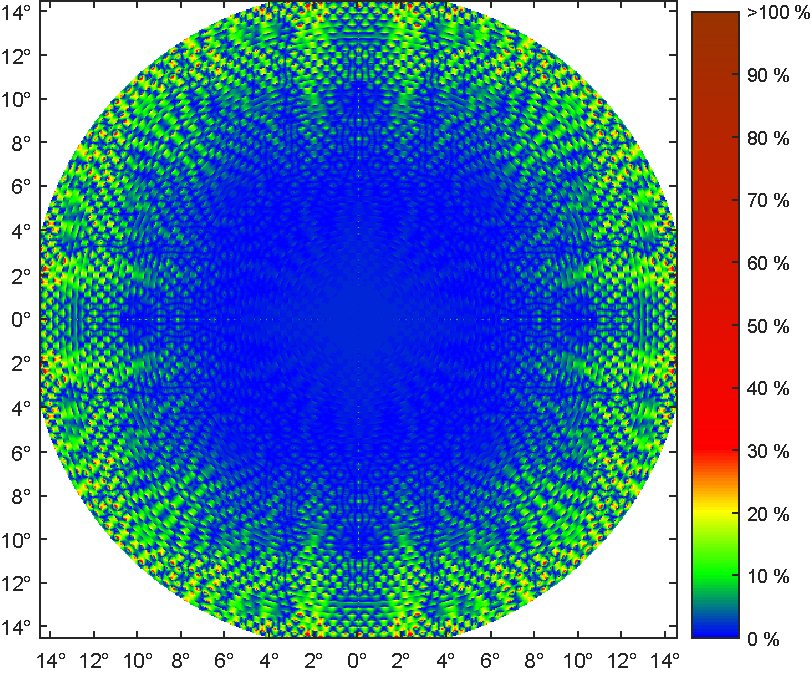
\includegraphics[width=\textwidth]{images/fig_sim_relerror_thibault-r100-bd1e-3.pdf}
		\subcaption{Thibaults Multislice}
	\end{subfigure}\hfill
	\begin{subfigure}[b]{0.48\textwidth}
		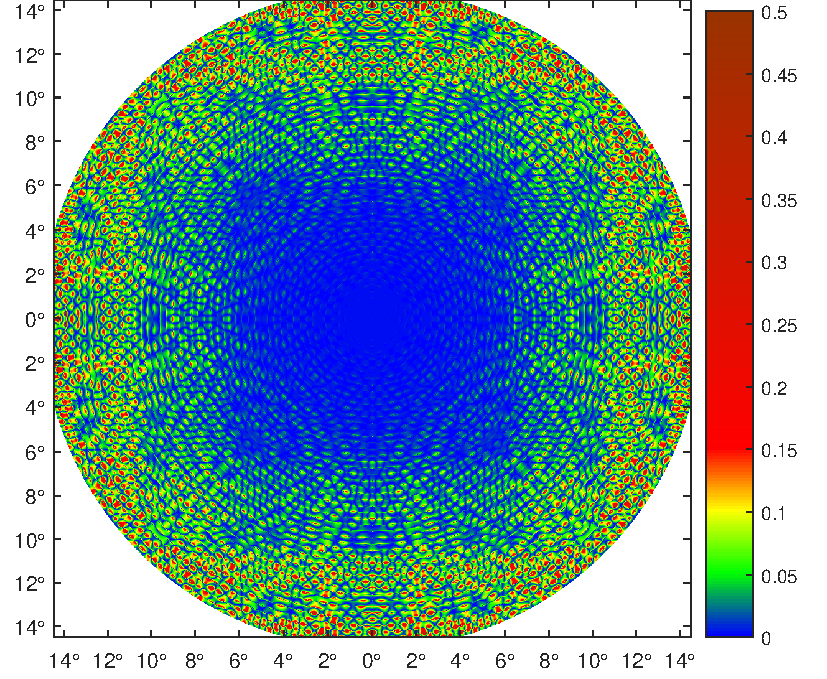
\includegraphics[width=\textwidth]{images/fig_sim_relerror_multislice-r100-bd1e-3.pdf}
		\subcaption{Multislice Propagation}
	\end{subfigure}
	\caption[Relativer Fehler der Simulationen]{Relative Abweichungen von Mie der simulierten Streubilder einer Kugel mit Radius \SI{100}{nm} bei $\beta=\delta=10^{-3}$. Es ist bei allen Simulationsmethoden der Trend zu ansteigenden Abweichung bei höheren Streuwinkeln sowie konzentrische Zonen höherer Abweichungen zu erkennen. Bei den hier verwendeten Parametern zeigt die Projektionsnäherung ein deutlich schlechteres Ergebnis als die Multislice Ansätze.}
	\label{fig:relerror}
\end{figure}

\clearpage
\begin{sidewaysfigure} %profile
	\centering
	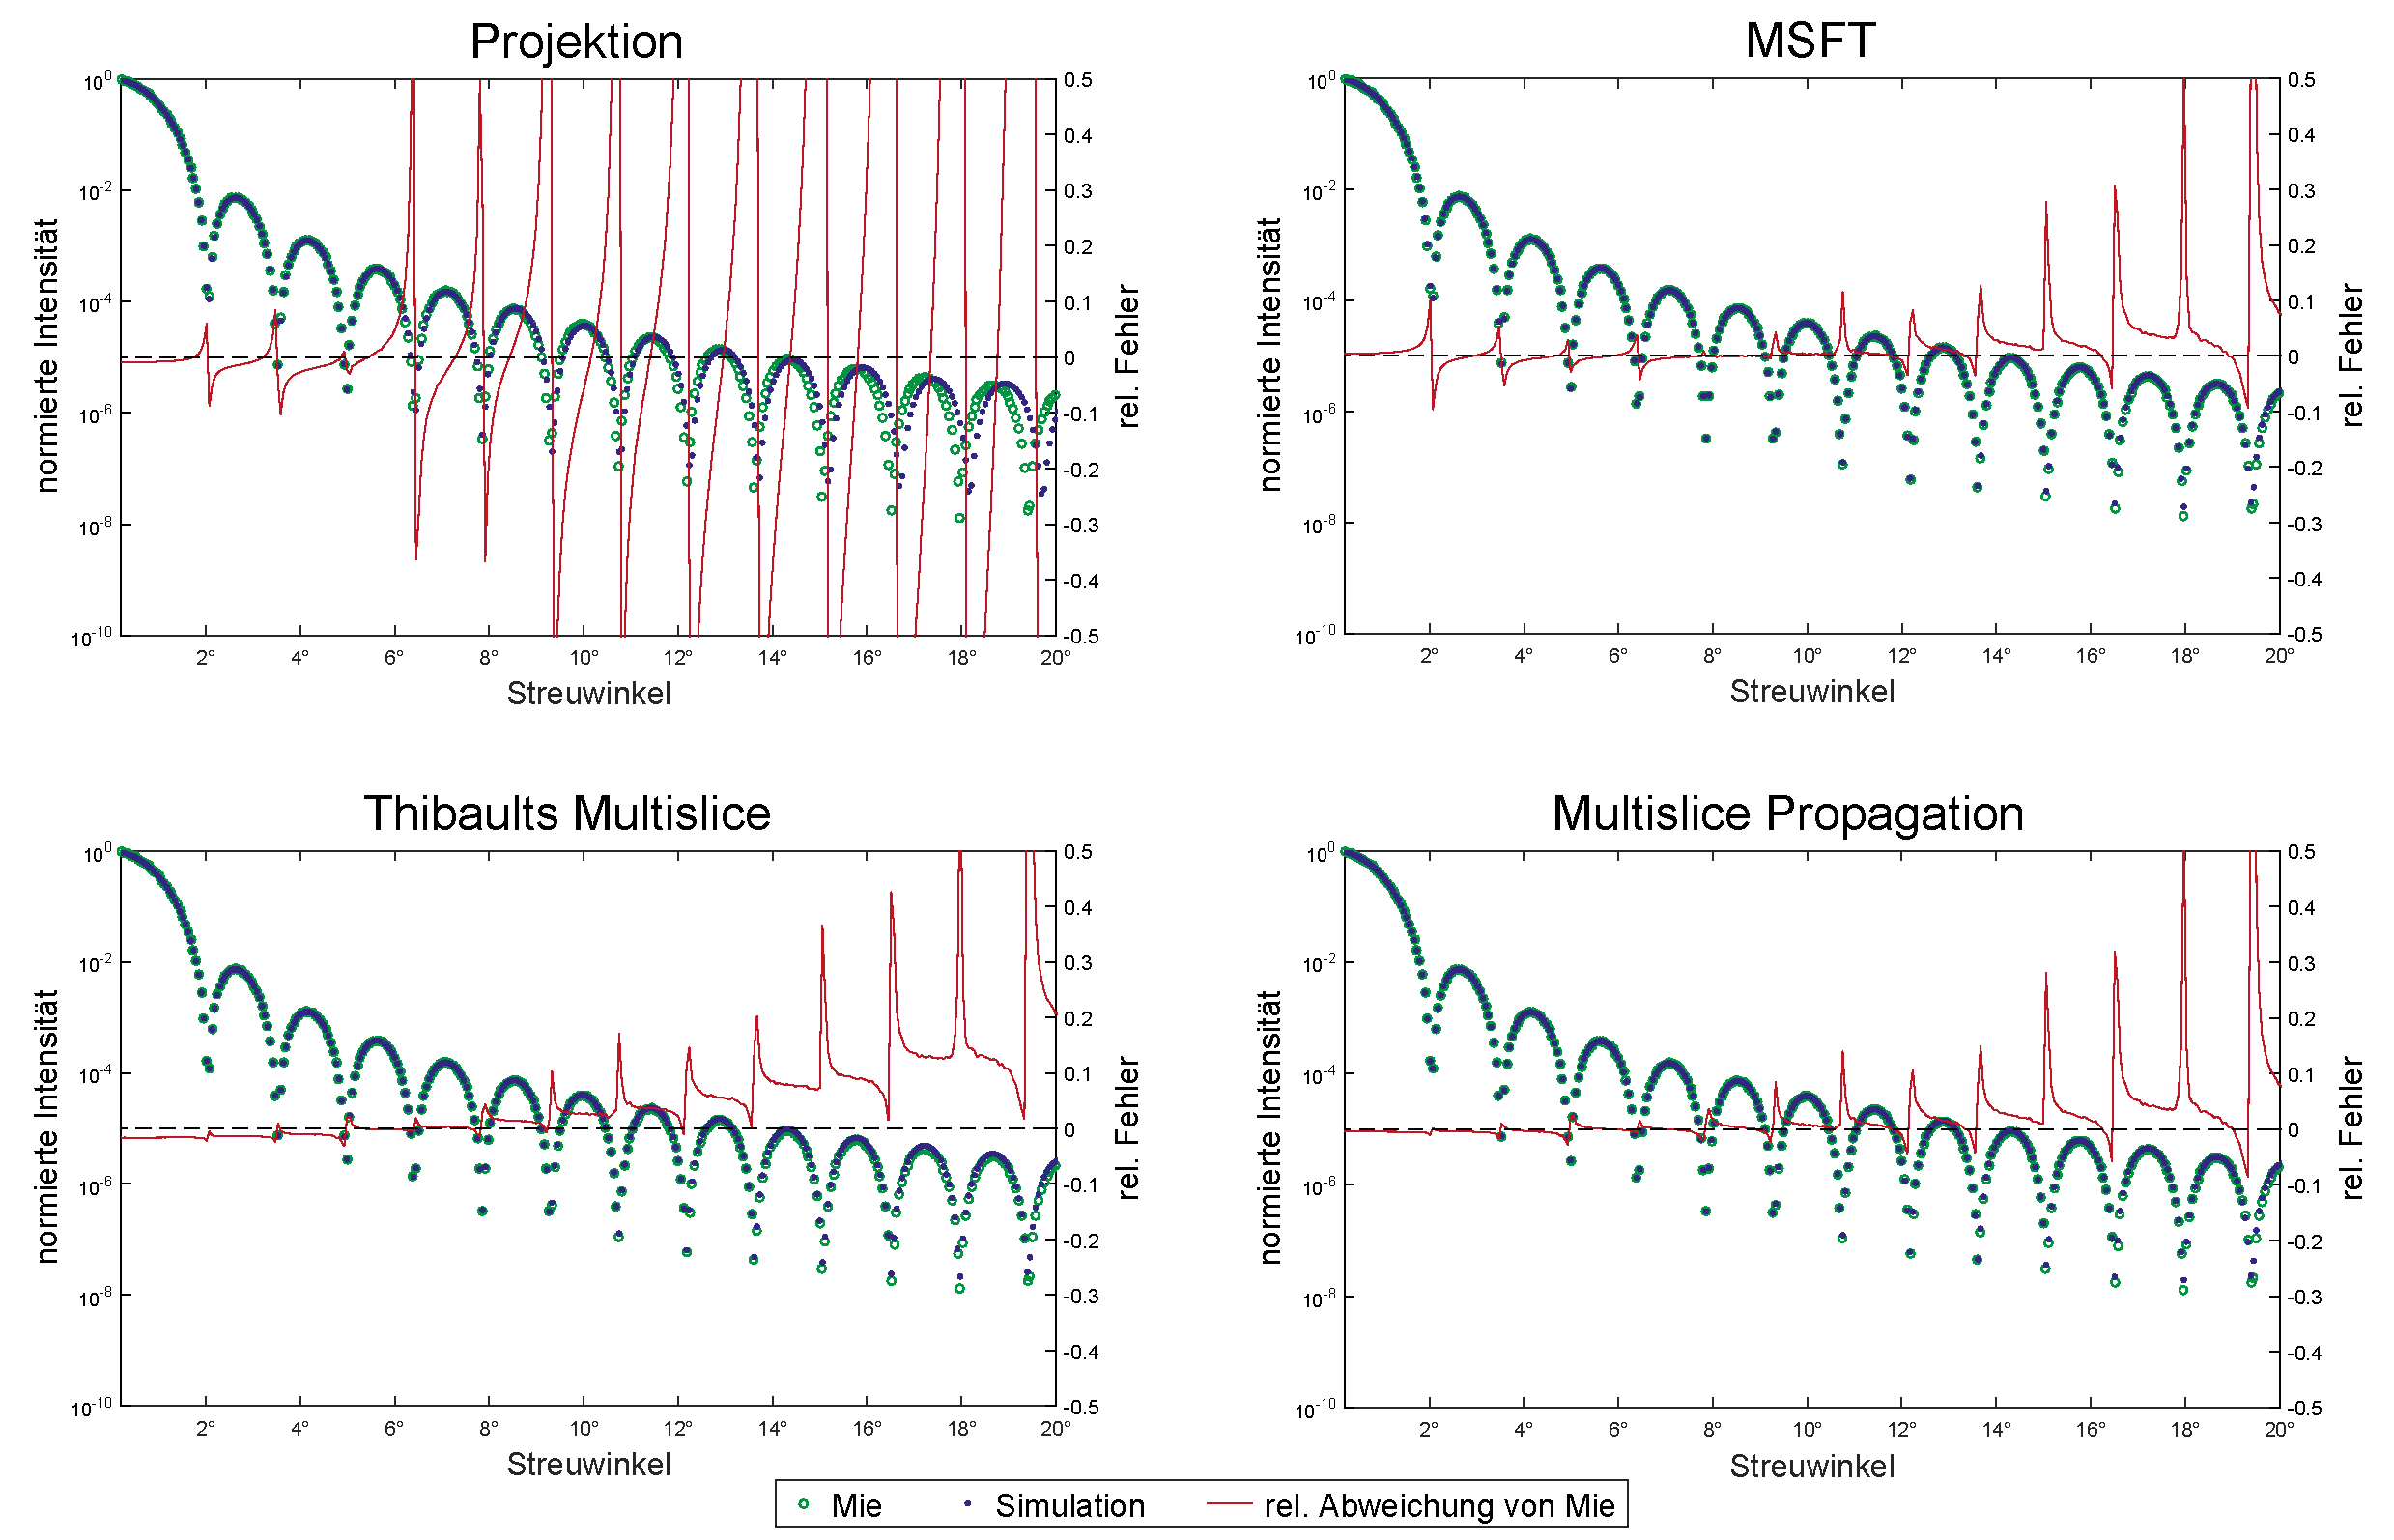
\includegraphics[width=1\textwidth]{images/fig_sim_profile.pdf}
	\captionsetup{width=0.95\textwidth}
	\caption[Radiale Profile]{Radiale logarithmierte Intensitätsprofile berechnet mit den verschiedenen Algorithmen sowie die relative Abweichung von Mie für eine Kugel mit Radius \SI{20}{nm} und $\beta,\delta$=$10^{-4}$. Es ist bei kleinen Streuwinkeln eine gute Übereinstimmung aller Algorithmen zu erkennen, bei höheren Winkeln versagt die Projektion. Über den gesamten Bereich besitzt bei diesen Parametern die Multislice Propagation die beste Übereinstimmung. Die relativen Fehler der Simulationen sind in den Intensitätsminima aufgrund der dort deutlich abfallenden Referenzintensität bei allen Verfahren stärker ausgeprägt.}
	\label{fig:profil}
\end{sidewaysfigure}
\clearpage

\begin{figure} %parameter variation
	\centering
	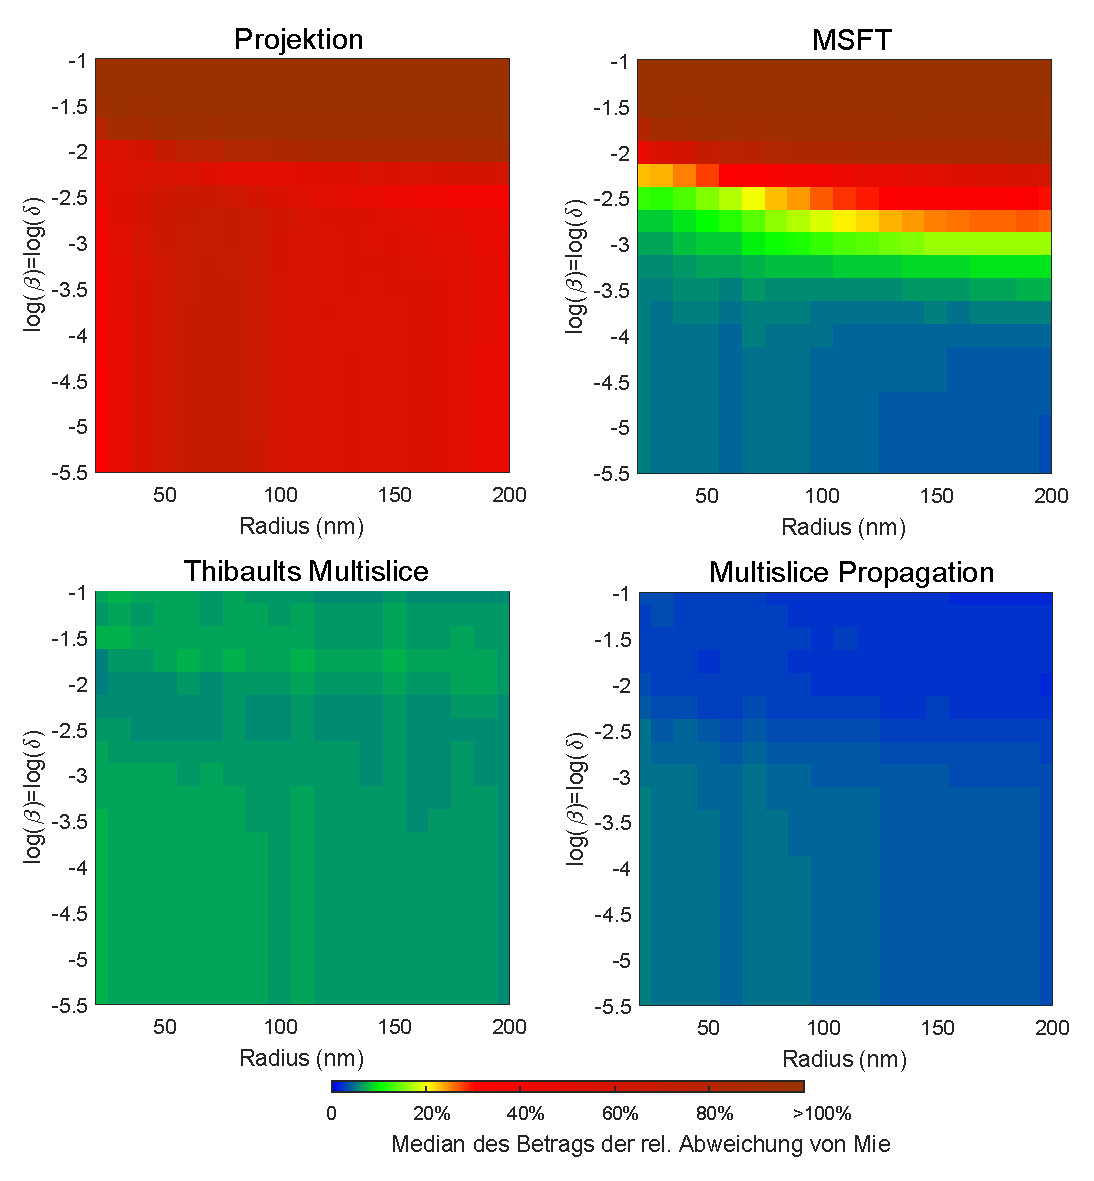
\includegraphics[width=1\textwidth]{images/fig_sim_var.pdf}
	\caption[Gültigkeit der Simulationsalgorithmen]{Zur Entscheidung bei welchen Radien und welchen Abweichungen der Brechzahl vom Vakuum die Simulationen noch valide sind, ist die mediane, relative Abweichung bis 20° von Mie über den Parametern aufgetragen. Es sind somit die Bereiche erkennbar, in denen der jeweilige Simulationsalgorithmus valide Ergebnisse liefert. Es ist insbesondere zu erkennen, dass bei größeren Brechzahlen sowie größeren Abweichungen von der Vakuumbrechzahl \textit{MSFT} nur eingeschränkt valide ist, sowie dass die \textit{Multislice Propagation} und \textit{Thibaults Multislice} über den gesammten dargestellten Bereich gute Ergebnisse liefern. Parameter: $\Delta x=\sfrac{\lambda}{2}$, $\Delta z$ und $\sfrac{\lambda}{8}$ und N=2048.}
	\label{fig:variation}
\end{figure}

Mit der \textit{Multislice Propagation} ist somit ein effizienter, schichtweise arbeitender Algorithmus gefunden, der sich für die Simulation synthetischer Streubilder eignet.


\section{Streubilder komplexer Objekte}
Neben der bislang zur Validierung erfolgten Berechnung von Streubildern von Kugeln eignen sich die Simulationsalgorithmen auch zur Berechnung der Austrittswellen und Streubilder hinter anderen, komplexeren Objekten.

Als interessante Testszene wird das in \fref{fig:komplexmodel} dargestellte Modell einer wassergefüllte ikosaederförmige Lecithin-Membran (Außenradius \SI{375}{nm}, Dicke \SI{25}{nm}) um deren Mittelpunkt vier kleinere, DNA gefüllte Kugeln (Radius \SI{90}{nm}) in den Eckpunkten eines Tetraeders angeordnet sind als biologisches Objekt betrachtet. Als Referenz dient ein disjunktes Xenon-Dodekaeder mit Außenradius \SI{100}{nm}. Die komplexen Brechzahlen der simulierten Materialien sind in \fref{tab:brechzahl} aufgeführt~\cite{henke,bergh2008,milo2015}. Die für diese Szene berechnete komplexe Austrittswelle ist in \fref{fig:komplexexit} gezeigt. Es sind sowohl die Wirkung der Absorption in Form der Intensitätsabnahme hinter den Streuobjekten, wie auch der Brechung in Form einer geringen Intensitätszunahme um die Streuobjekte sowie einer Phasenänderung zu erkennen. Das zugehörige Streubild ist in \fref{fig:komplexscatter} gezeigt und stellt das Ergebnis der Bemühungen synthetische Streubilder zu erstellen dar. Im Folgenden wird dies für den Vergleich der Rekonstruktionsansätze genutzt, indem deren Eignung zur Rekonstruktion der Austrittswelle betrachtet wird.

  
\begin{table}[b]
	\begin{minipage}[b]{.64\textwidth }%
	 	\begin{small}
 			\begin{tabular}{lll}
 				\hline
 				Material													&Brechzahl bei \SI{1}{nm}~\cite{henke}\\
 				\hline
 				Lecithin (\chem{C_{44}H_{82}NO_8P})~\cite{milo2015}			&$1-(1.69-0.12i)\times10^{-4}$			\\ 					
 				Wasser														&$1-(1.55-0.18i)\times10^{-4}$			\\
 				Protein (\chem{H_{86}C_{52}N_{13}O_{15}S})~\cite{bergh2008}	&$1-(2.03-0.16i)\times10^{-4}$			\\
 				Xenon-Cluster												&$1-(2.54-1.46i)\times10^{-4}$			\\
 				\hline
 			\end{tabular}
		\end{small}
		\centering
		\caption[Für die Berechnung der komplexen Austrittswelle verwendete Materialien]{Brechzahlen der verwendeten Materialien}   \label{tab:brechzahl}
	\end{minipage}
	\begin{minipage}[b]{.35\textwidth}
				\hspace*{0pt}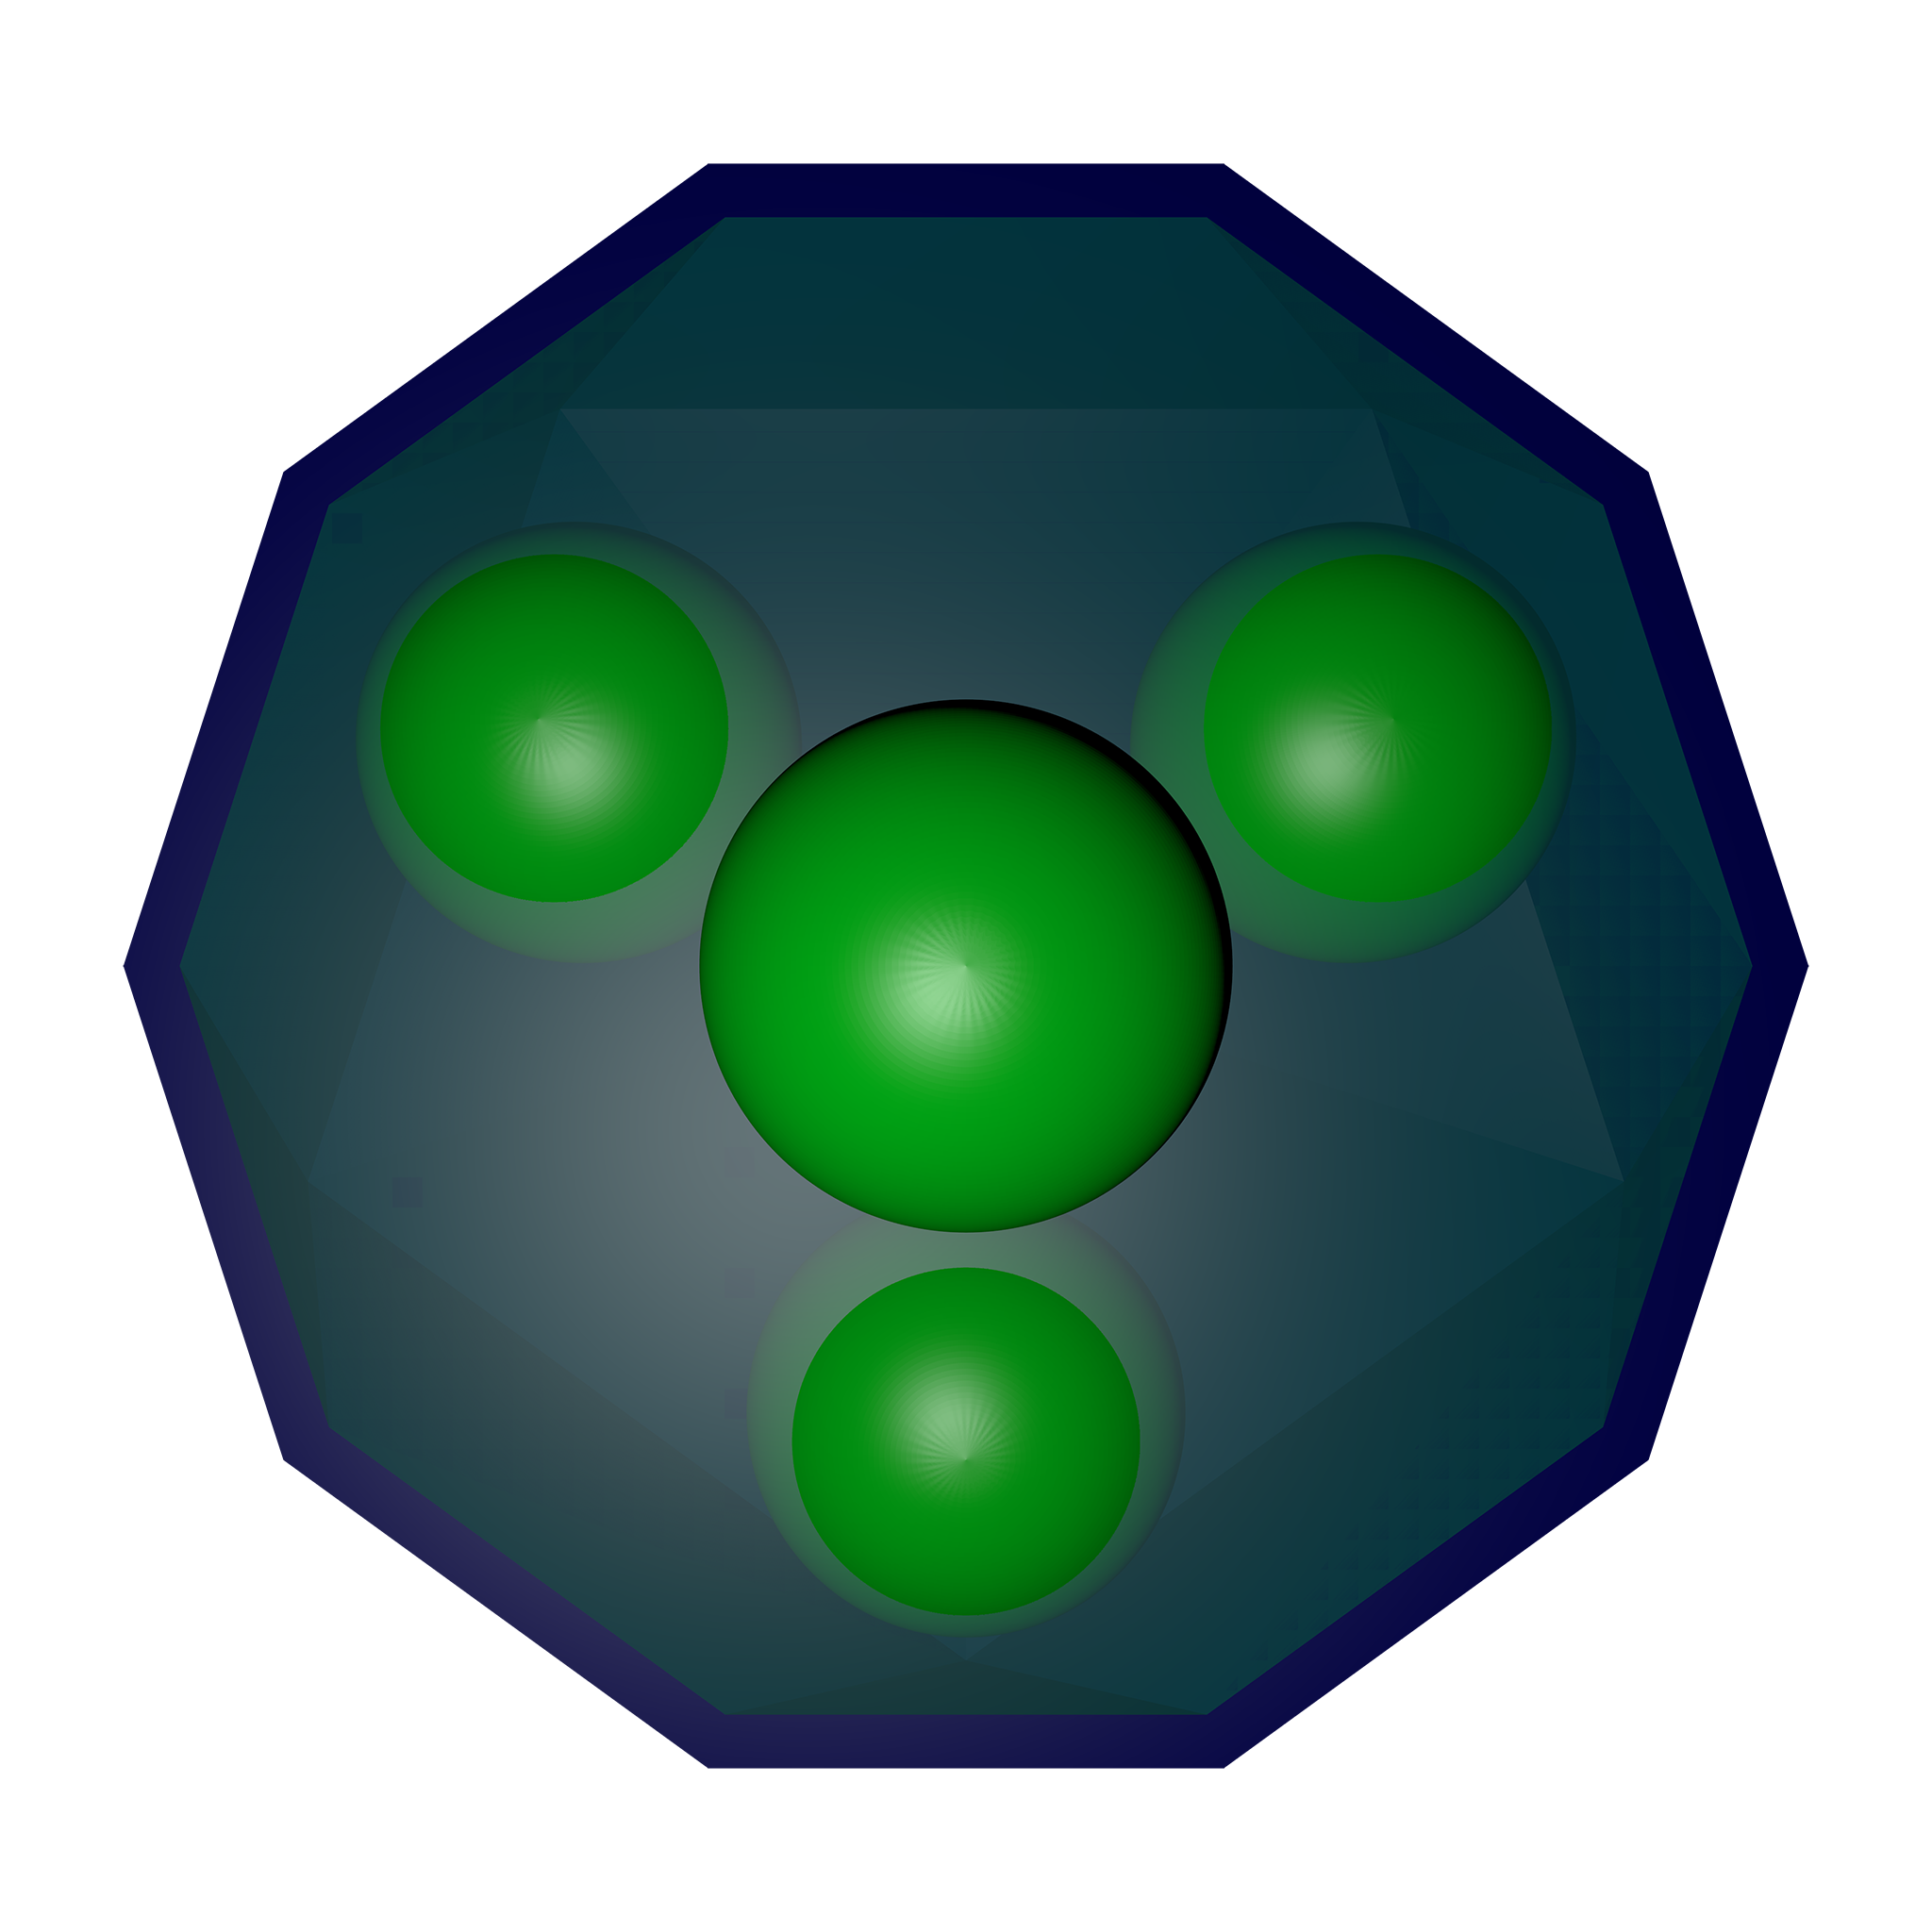
\includegraphics[width=.8\textwidth]{images/scene.png}%
				\captionof{figure}{3D-Modell\label{fig:komplexmodel}}%
	\end{minipage}
	\par\bigskip
\end{table}


\begin{figure}[b] %exitwave und scatter
	\begin{subfigure}[b]{0.45\textwidth}
		\setbox1=\hbox{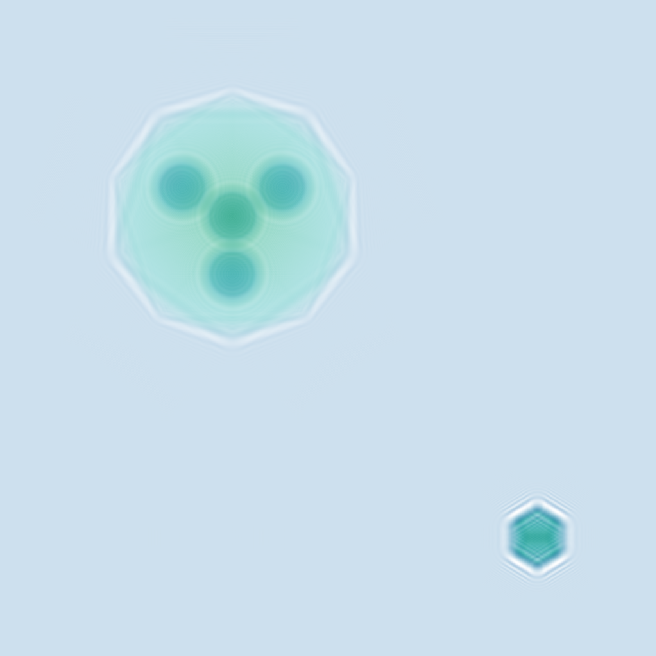
\includegraphics[width=\textwidth]{images/fig_simholo_v2_exitwave.png}}
		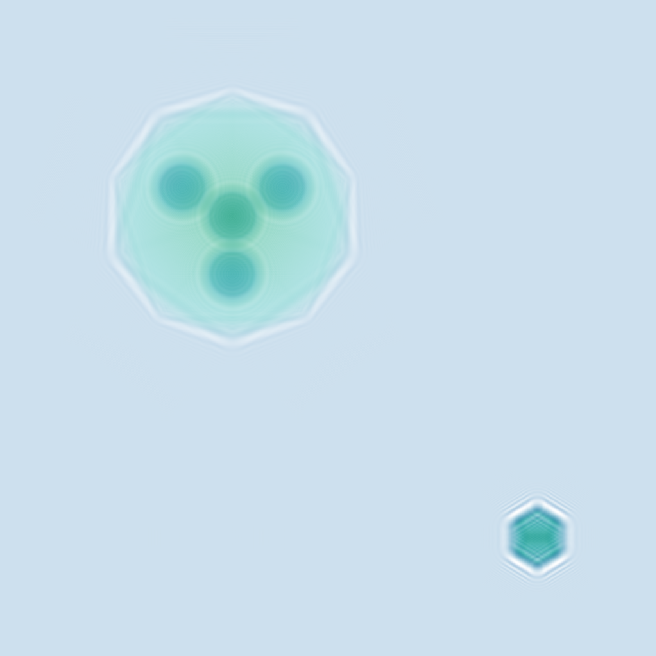
\includegraphics[width=\textwidth]{images/fig_simholo_v2_exitwave.png}\llap{\makebox[\wd1][l]{\includegraphics[width=0.5\textwidth]{images/fig_simholo_v2_exitwave_cw.pdf}}}
		\caption{Austrittswelle}
		\label{fig:komplexexit}
	\end{subfigure}	\hfill
	\begin{subfigure}[b]{0.45\textwidth}
		\setbox1=\hbox{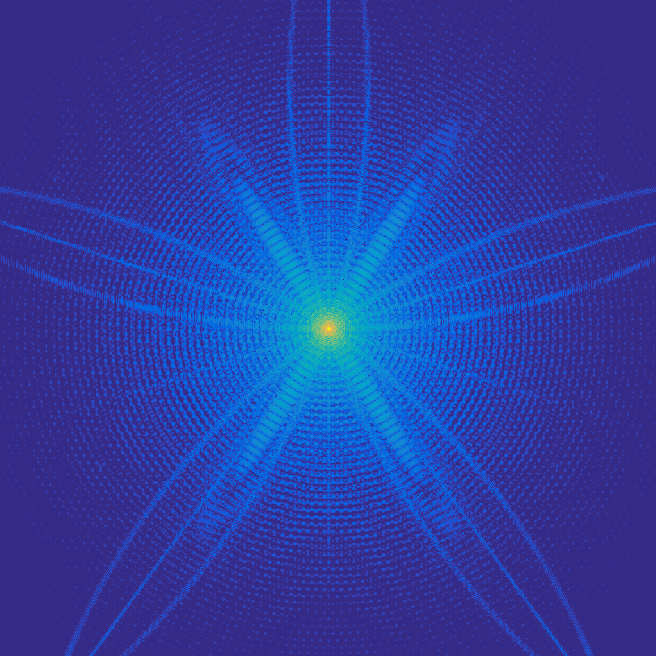
\includegraphics[width=\textwidth]{images/fig_simholo_v2_scatter.png}}
		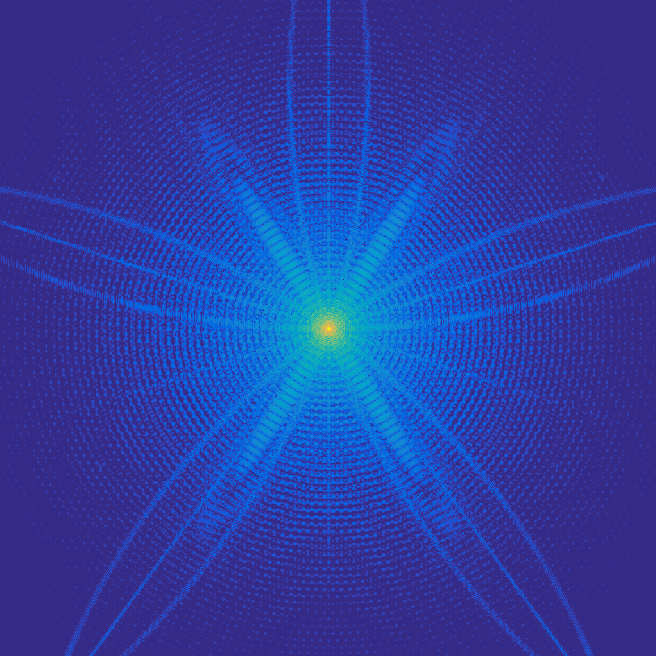
\includegraphics[width=\textwidth]{images/fig_simholo_v2_scatter.png}\llap{\makebox[\wd1][l]{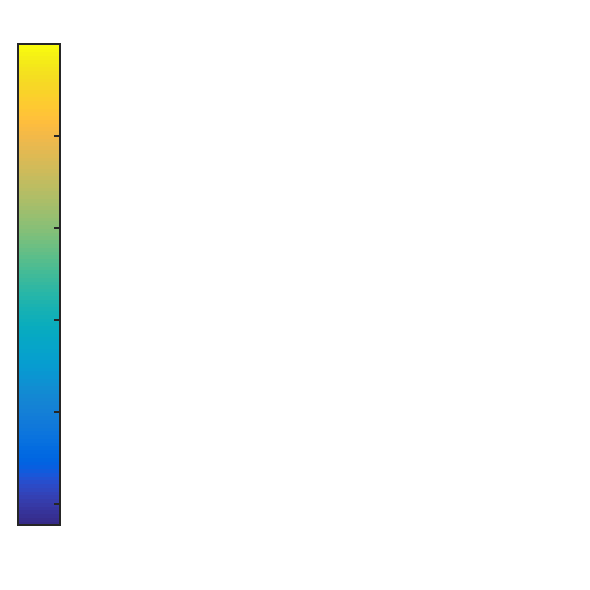
\includegraphics[width=0.5\textwidth]{images/fig_simholo_v2_scatter_cb.pdf}}}
			\caption{Streubild}
			\label{fig:komplexscatter}
	\end{subfigure}		
	\caption[Austrittswelle und Streubild eines komplexen Objektes]{Austrittswelle und logarithmiertes Streubild eines komplexen Objektes. Bei der Austrittswelle ist die relative Intensität bezüglich der Eintrittswelle über die Helligkeit dargestellt, die Phase über den Farbton.}
	\label{fig:komplex}
\end{figure}
